
%% limited to 12 pages, to format use commands:

%% pdflatex main
%% bibtex main
%% pdflatex main
%% pdflatex main

%% view main.pdf with your favorite pdf viewer....

%% OK, for the ACM SIG formatting we have to use latex and dvips to get the
%% desired output.  in particular they suggest the following dvips command be
%% used:

%%ps2pdf14 -dPDFSETTINGS=/prepress pads028-wilsey.ps

\documentclass{sig-alternate}

\usepackage{amsmath}

\begin{document}

%%\conferenceinfo{SIGSIM-PADS'13,} {May 19--22, 2013, Montréal, Québec, Canada.} 
\CopyrightYear{2015} 
%%\crdata{978-1-4503-1920-1/13/05} 
\clubpenalty=10000 
\widowpenalty = 10000

\title{Experiments with Hardware-based Transactional Memory in Parallel Simulation}

\numberofauthors{2} 

\author{
%% \alignauthor
%% Joshua Hay \\
%%        \affaddr{Intel Corporation}\\
%%        \affaddr{Oregon}\\
%%        \email{sounak.besu@gmail.com}
%% \alignauthor
%% Philip A. Wilsey \\
%%        \affaddr{Dept of of Electrical Engineering and Computing Systems}\\
%%        \affaddr{Cincinnati, OH  45221-0030}\\
%%        \email{wilseypa@gmail.com}
}

\maketitle

\begin{abstract}

Transactional memory is a concurrency control mechanism that dynamically determines when
threads may safely execute critical sections of code.  It provides the performance of
fine-grained locking mechanisms with the simplicity of coarse-grained locking mechanisms.
With hardware based transactions, the protection of shared data accesses and updates can
be evaluated at runtime so that only true collisions to shared data force serialization.

This paper explores the use of transactional memory as an alternative to conventional
synchronization mechanisms for managing the pending event set in a Time Warp synchronized
parallel simulator.  In particular, we explore the application of Intel's hardware-based
transactional memory (TSX) to manage shared access to the pending event set by the
simulation threads.  Comparison between conventional locking mechanisms and transactional
memory access is performed to evaluate each within the \textsc{warped} Time Warp
synchronized parallel simulation kernel.  In this testing, evaluation of both forms of
transactional memory found in the Intel Haswell processor (HLE and RTM) are evaluated.
The results show that RTM generally outperforms conventional locking mechanisms and that
HLE provides consistently better performance than conventional locking mechanisms, in some
cases as much as 27\%.

\end{abstract}

\category{D.1.3}{Programming Techniques}{Concurrent Programming}[parallel
  programming, distributed programming]

\category{I.6.8}{Simulation and Modeling}{Types of Simulation}[parallel,
  distributed, discrete event]

\terms{Algorithms, Performance}

\keywords{Transactional memory, parallel simulation, optimistic synchronization, pending event set}

\section{Introduction}\label{intro} 

The advent of multi-core processors introduced a new avenue for increased software
performance and scalability through multi-threaded programming.  However, this avenue came
with a toll: the need for synchronization mechanisms between multiple threads of
execution, especially during the execution of critical sections.  By definition, a
critical section is a segment of code accessing a shared resource that can only be
executed by one thread at any given time \cite{os_concepts}.  For example, consider a
multi-threaded application that is designed to operate on a shared two-dimensional array.
For the sake of simplicity, the programmer uses coarse-grained locking mechanisms to
control access to the critical section, \emph{e.g.,} a single atomic lock for the entire
structure.  The critical section reads a single element, performs a calculation, and
updates the element of the array.  Once a thread enters the critical section, it locks all
other threads out of the entire array until it has completed its task, thus forcing the
collection of threads to essentially execute sequentially through the critical section
even when they are accessing completely independent parts of the array.  This results in
lock contention, and consequently negatively impacts performance, as threads must now wait
for the currently executing thread to relinquish access to the shared resource.
Programmers can employ more fine-grained locking mechanisms to expose concurrency, such as
locking individual rows or even individual elements in the previous example.  However,
this approach is vastly more complicated and error prone \cite{sle_rajwar}; this approach
requires the programmer to define and maintain a separate lock for each row or each
element.  Unfortunately, programmers are limited to using static information to decide
when threads must execute a critical section regardless of whether coarse-grained or
fine-grained locking is used.

Transactional memory (TM) is a concurrency control mechanism that attempts to eliminate
the static sequential execution of a critical section by dynamically determining when
accesses to shared resources can be executed concurrently \cite{sle_rajwar}.  In the
above example, instead of using locks, the programmer identifies the critical section
as a transactional region (hereafter, the terms \emph{critical region} and
\emph{transaction} will be used interchangeably).  As the threads enter the transactional
region, they attempt to ``atomically'' execute the critical section.  The TM system
records memory accesses as the transactions execute and finds that the transactions
operate on independent regions of the data structure, \emph{i.e.,} there are no
conflicting memory accesses.  Instead of being forced to execute sequentially by the
conventional locking mechanisms, the threads are allowed to safely execute the critical
section concurrently.  Transactional memory is analogous to traffic roundabouts whereas
conventional synchronization mechanisms are analogous to conventional traffic lights
\cite{neuling_vid}.

Transactional memory operates on the same principles as database transactions
\cite{tm_2nd}.  The processor atomically commits \emph{all} memory operations of a
successful transaction or discards \emph{all} memory operations if the transaction should
fail (a collision to the updates by the multiple threads occurs).  In order for a
transaction to execute successfully, it must be executed in isolation, \emph{i.e.,}
without conflicting with other transactions/threads memory operations.  This is the key
principle that allows transactional memory to expose untapped concurrency in
multi-threaded applications.

One problem space that could benefit from transactional memory is that Parallel Discrete
Event Simulation (PDES).  A key challenge area in PDES is the need for contention-free
pending event set management solutions \cite{dickman}.  Transactional memory can help
alleviate contention for this shared structure and potentially expose additional untapped
concurrency in the simulation's execution.

This paper explores the use of transactional memory to manage the pending event set
schedule queue in the \textsc{warped} parallel simulation kernel.  In particular, we will
integrate the hardware-based transactional memory primitives from the Intel Haswell
platform to manage the pending event set data structures of the \textsc{warped} parallel
discrete event simulation engine.  While \textsc{warped} has multiple shared data
structures in the kernel, the focus of this work is on the pending event set.  It is the
primary bottleneck in PDES applications, and hence the primary motivation for this study.

The remainder of this paper is organized as follows.  Section \ref{background} provides a
general overview of transactional memory.  It gives some examples of other TM
implementations and discusses why they do not work as well as TSX.  It provides examples
of related studies.  Finally, it provides an overview of how TSX works and how it is
implemented in software.  Section \ref{warped} provides some background of the PDES
problem space.  It introduces \textsc{warped} and some of the implementation details
relevant to this study.  Previous studies with the \textsc{warped} pending event set are
also briefly discussed.  Section \ref{tsx} discusses how TSX is incorporated into the
\textsc{warped} pending event set implementation.  It also provides a brief
overview of the critical sections utilizing TSX and why TSX will be beneficial.
Section \ref{eval} presents the experimental results of this research for several
different simulation configurations.  Finally, Section \ref{conclude} contains some
concluding remarks.


\section{Background}\label{background}

This section provides a high level explanation of how transactional memory operates.  It
then introduces other implementations, as well as reasons why they were not explored in
this study.  Next, it provides some examples of related studies with transactional memory,
specifically the implementation used in this study.  Finally, it provides an overview of
Intel's implementation, Transactional Synchronization Extensions (TSX) and how the
programmer can develop TSX enabled multi-threaded applications.

\subsection{Transactional Memory Overview}

Transactional memory (TM) is a concurrency control mechanism that dynamically determines
when two or more threads can safely execute a critical section \cite{sle_rajwar}.  The
programmer identifies a transactional region, typically a critical section, for
monitoring.  When the transaction executes, the TM system, whether it is implemented in
hardware or software, tracks memory operations performed within the transactional region
to determine whether or not two or more transactions conflict with one another,
\emph{i.e.,} if any memory accesses conflict with one another.  If the threads do not
conflict with one another, the transactions can be safely and concurrently executed.  If
they do conflict, the process must abort the transaction and execute the critical section
non-transactionally, \emph{i.e.,} by serializing execution of the critical section with
conventional synchronization mechanisms.

%% JOSH: review this rewritten paragraph and verify/correct it accordingly.
%%As a transaction is executed, the processor buffers the memory write operations and
%%commits them only when the transaction is complete and safe access has been determined.
%%Safe access is determined by the processor core by recording the set memory read addresses
%%(called the \emph{read-set}) and memory write addresses (called the \emph{write-set}) from
%%the instructions in the transaction.  During the time of the transaction memory addresses
%%of instructions executed by other concurrently executed threads are also recorded.  If
%%there is an intersection of the addresses from the transaction with addresses from any of
%%the concurrently executed threads, the transaction aborts (safe access did \emph{not}
%%occur).  Upon completing a transaction with safe access, the transaction will atomically
%%commit all of the buffered memory operations, henceforth referred to simply as a
%%\emph{commit}.

%% JOSH: here's a question, what happens if the code accesses a shared memory region
%% outside of a transaction (say it reads it); does this get considered in the validity of
%% the transaction?  or would it simply commit?

%% Dr. Wilsey: It is my understanding that ANY memory operation performed
%% during transactional execution is tracked by the TM system.  So if a shared
%% memory region is accessed outside of a transaction (which I'm not 100% sure what
%% you mean by that). it will still be added to the transactions read-set for
%% conflict detection.

%% JOSH: outside of a transaction means exactly that, a memory reference that is not
%% contained within a transction (critical region).  
%%
%% ok, now that we have established that the tracking of memory references outside of a
%% transaction do indeed happen, i have two comments:
%% (1) you should revise the prose below to make that fact more clear in your description
%%     of (at least the haswell implementation of) transactional memory.
%% (2) would there be any performance benefit of skipping the use of the transaction
%%     operations for a read to a shared variable?  if so, what can/should we say about
%%     that?

%% If that shared variable is ever written to, I don't see how you could skip the
%% transaction operations or any synchronization.  That's the only way to ensure
%% consistent data/results.  And if it's never written to, then it doesn't need to be a
%% critical section/transactional region in the first place.  I would imagine the commit
%% overhead is substantially less when only read operations are performed, but Intel
%% didn't provide that level of implementation detail.

%% JOSH: yes certainly we would have to have all shared data writes in a critical region,
%% i was just asking about the read operations.

As a transaction is executed, the memory operations performed within the transaction are
buffered, specifically write operations.  Write operations will only be fully committed
when the transaction is complete and safe access has been determined.  Safe access is
determined by comparing the set of addresses each transaction reads from (called the
\emph{read-set} and the set of addresses each transaction writes to (called the
\emph{write-set}).  Each transaction builds its own read-set and write-set as it executes.
While a thread is executing transactionally, any memory operation performed by any other
thread is checked against the read-set and write-set of the transactionally executing
thread to determine if any memory operations conflict.  The other threads can be executing
either non-transactionally or transactionally.  If the transaction completes execution and
the TM system has not detected any conflicting memory operations, the transaction
atomically commits all of the buffered memory operations, henceforth referred to simply as
a \emph{commit}.

Whenever safe access does not occur, the transaction cannot safely continue execution.
This is referred to as a \emph{data conflict} and only occurs if: (i) one transaction
attempts to read a location that is part of another transaction's write-set, or (ii) a
transaction attempts to write a location that is part of another transaction's read-set or
write-set \cite{intel_prog_ref}.  Once a memory location is written to by a transaction,
it cannot be accessed in any way by any other transaction; any access by any other
transaction results in a race condition.  If such a situation arises, all concurrently
executing transactions will abort execution, henceforth referred to simply as an
\emph{abort}.

By definition, a transaction is a series of actions that appears instantaneous and
indivisible possessing four key attributes: (1) atomicity, (2) consistency, (3) isolation,
and (4) durability \cite{tm_2nd}.  TM operates on the principles of database transactions.
The two key attributes for TM are atomicity and isolation; consistency and durability must
hold for all multi-threaded operations in multi-threaded applications.  Atomicity is
guaranteed if: (1) all memory operations performed within the transaction are completed
successfully, or (2) it appears as if the performed memory operations were never attempted
\cite{tm_2nd}.  Isolation is guaranteed by tracking memory operations as the transactions
execute and aborting if any memory operations conflict.  If both atomicity and isolation
can be guaranteed for all memory operations performed within a critical section, that
``critical section'' can be executed concurrently \cite{sle_rajwar}.

In the case of a commit, the transaction has ensured that its memory operations are
executed in isolation from other threads and that \emph{all} of its memory operations are
committed, thus satisfying the isolation and atomicity principles.  Note that only at this
time will the memory operations performed within the transaction become visible to other
threads, thus satisfying the appearance of instantaneousness.  In the case of an abort due
to a data conflict, it is clear that the isolation principle has been violated.  It should
be noted that transactions can abort for a variety of reasons depending on the
implementation \cite{intel_opt_man,chung_amd}, but the primary cause is data conflicts.
Upon abort, all memory operations are discarded to maintain atomicity.

\subsection{Related Studies}

There have been many implementations of TM systems since its conception, mostly in software
\cite{yoo_tsx,chitters_tsx,rock_dice,chung_amd,blue_wang,quake_stm,stm_cascaval}.  As the
name suggests, Software Transactional Memory (STM) systems implement the memory tracking,
conflict detection, write buffering and so on in software.  Most systems are
implementation specific, but memory tracking is typically done through some form of
logging.  While this allows transactional memory enabled applications to be executed on a
variety of platforms, performance usually suffers.  Gajinov \emph{et al} performed a study
with STM by developing a parallel version of the Quake multi-player game server from the
ground up using OpenMP parallelizations pragmas and atomic blocks \cite{quake_stm}.  Their
results showed that the logging overhead required for STM resulted in execution times that
were 4 to 6 times longer than the sequential version of the server.  In general, STM has
been found to result in significant slowdown \cite{stm_cascaval}.  Although STM is more
widely available than HTM, its use in this this study was dismissed due to the significant
performance penalty.

Hardware Transactional Memory (HTM) provides the physical resources necessary to implement
transactional memory effectively.  Many chip manufacturers have added, or at least sought
to add, support for HTM in recent years.  IBM released one of the first commercially
available HTM systems in their Blue Gene/Q machine \cite{blue_wang}.  Even though they
found that this implementation was an improvement over STM, it still incurred significant
overhead.  AMD's Advanced Synchronization Facility and Sun's Rock processor included
support for HTM \cite{chung_amd,rock_dice}.  However, AMD has not released any HTM enabled
processors and Sun's Rock processor was canceled after Sun was acquired by Oracle.

With the release of Intel's Haswell generation processors, Intel's Transactional
Synchronization Extensions (TSX) is currently the only widely available commercial
HTM-enabled system.  Numerous studies have already been performed with TSX, primarily
evaluating its performance capabilities.  Chitters \emph{et al} modified Google's write
optimized persistent key-value store, LevelDB, to use TSX based synchronization instead of
a global mutex.  Their implementation shows 20-25\% increased throughput for write-only
workloads and increased throughput for 50\% read / 50\% write workloads
\cite{chitters_tsx}.  Wang \emph{et al} studied the performance scalability of a
concurrent skip-list using TSX Restricted Transactional Memory (RTM).  They compared the
TSX implementation to a fine-grain locking implementation and a lock-free implementation.
They found that the performance was comparable to the lock-free implementation without the
added complexity \cite{wang_tsx}.  Yoo \emph{et al} evaluated the performance of TSX using
high-performance computing (HPC) workloads, as well as in a user-level TCP/IP stack.  They
measured an average speed up of 1.41x and 1.31x respectively \cite{yoo_tsx}.  The decision
to use Intel's TSX for this research was based on its wide availability and the
performance improvements observed in other studies.

\subsection{Transactional Synchronization Extensions (TSX)}

Intel's Transactional Synchronization Extensions (TSX) is an extension to the x86
instruction set architecture that adds support for HTM.  TSX operates in the L1 cache
using the cache coherence protocol \cite{intel_opt_man}.  It is a best effort
implementation, meaning it does not guarantee transactions will commit
\cite{intel_prog_ref}.  TSX has two interfaces: (1) Hardware Lock Elision (HLE), and (2)
Restricted Transactional Memory (RTM).  While both operate on the same principles of
transactional memory, they have subtle differences.  This section discusses some of the
implementation details of TSX as well as how the programmer utilizes TSX.

The \emph{\textbf{Hardware Lock Elision}} (HLE) interface is a legacy-compatible interface
introducing two instruction prefixes, namely: \texttt{XACQUIRE} and \texttt{XRELEASE}.

The \texttt{XACQUIRE} prefix is placed before a locking instruction to mark the beginning
of a transaction.  \texttt{XRELEASE} is placed before an unlocking instruction to mark the
end of a transaction.  These prefixes tell the processor to elide the write operation to
the lock variable during lock acquisition/release.  When the processor encounters an
\texttt{XACQUIRE} prefixed lock instruction, it transitions to transactional execution.
Specifically, it adds the lock variable to the transaction's read-set instead of issuing
any write requests to the lock \cite{intel_prog_ref}.  To other threads, the lock will
appear to be free, thus allowing those threads to enter the critical section and execute
concurrently.  All transactions can execute concurrently as long as no transactions abort
and explicitly write to the lock variable.  If that were to happen, a data conflict
technically occurs --- one transaction writes to a memory location (the lock) that is part
of another transaction's read-set.

The \texttt{XRELEASE} prefix is placed before the instruction used to release the lock.
It also attempts to elide the write associated with the lock release instruction.  If the
lock release instruction attempts to restore the lock to the value it had prior to the
\texttt{XACQUIRE} prefixed locking instruction, the write operation on the lock is elided
\cite{intel_prog_ref}.  It is at this time that the processor attempts to commit the
transaction.  

However, if the transaction aborts for any reason, the region will be re-executed
non-transactionally.  If the processor encounters an abort condition, it will discard all
memory operations performed within the transaction, return to the locking instruction, and
resume execution without lock elision, \emph{i.e.,} the write operation will be performed
on the lock variable.  If another thread is executing the same transactional region, those
transactions will also abort.  The aborted transaction thread performs an explicit write
on the lock, resulting in a data conflict for any other transaction as the lock variable
is part of the other transaction's read-set.  The re-execution of the critical section
using conventional synchronization is necessary to guarantee forward progress
\cite{intel_prog_ref}.

%% An example of a standard locked critical section using the x86 atomic exchange
%% instruction is shown in Figure~\ref{fig:lock_interface} (as a reference for the TSX HLE
%% interfaces shown below).  The \texttt{\_\_atomic\_exchange\_n(type *ptr, type val, int
%% memmodel} intrinsic implements the atomic exchange operation as the name suggests.  It
%% writes \texttt{val} into \texttt{ptr} and returns the previous contents of
%% \texttt{ptr}.  The most important parameter is \texttt{memmodel}; it specifies
%% synchronization requirements between threads.  For instance, the \_\_ATOMIC\_ACQUIRE
%% memory model synchronizes the local thread with a release semantic store from another
%% thread \cite{gcc}.  Essentially, when another thread executes a lock release, the local
%% thread will execute the lock acquire.  The while loop further ensures the lock is free
%% before it is acquired (the while loop repeats the \texttt{\_\_atomic\_exchange\_n}
%% operation until the lock is acquired). 
%%
%%\begin{figure}
%%\begin{verbatim}
%%/* Acquire lock */
%%/* Loop until the returned value 
%%   indicates the lock was free */
%%while(__atomic_exchange_n(&lock, 1, __ATOMIC_ACQUIRE)):
%%
%%/* Begin executing critical section */
%%...
%%/* End critical section */
%%
%%/* Free lock */
%%__atomic_store_n(&lock, 0,__ATOMIC_RELEASE);
%%\end{verbatim}
%%    \caption{\textbf{Standard Atomic Lock Implementation}}\label{fig:lock_interface} 
%%\end{figure}

To enable HLE synchronization, the programmer merely adds the HLE memory models to the
existing locking intrinsics (Figure~\ref{fig:hle_interface}).  The
\_\_ATOMIC\_HLE\_ACQUIRE tells the thread to execute an \texttt{XACQUIRE} prefixed lock
acquire instruction when another thread releases the lock.  The combination of memory
models, \texttt{\_\_ATOMIC\_HLE\_ACQUIRE|\_\_ATOMIC\_ACQUIRE)} allows for the locking
instructions to be executed with or without elision.  The local thread can be synchronized
to a \texttt{XRELEASE} prefixed lock release instruction or a standard lock release
instruction.

\begin{figure}
\begin{verbatim}
/* Acquire lock with lock elision if possible */
/* Loop until the returned value 
   indicates the lock was free */
while(__atomic_exchange_n(&lock, 1, 
      __ATOMIC_HLE_ACQUIRE|__ATOMIC_ACQUIRE)):

/* Begin executing critical section/
   transactional region */
...
/* End critical section/transactional region */

/* Free lock with lock elision if possible */
__atomic_store_n(&lock, 0, 
         __ATOMIC_HLE_RELEASE|__ATOMIC_RELEASE);
\end{verbatim}
    \caption{\textbf{Generic HLE Software Implementation}}\label{fig:hle_interface}
\end{figure}

HLE is legacy compatible.  Code utilizing the HLE interface can be executed on legacy
hardware, but the HLE prefixes will be ignored \cite{intel_prog_ref} and the processor
will always perform the write operation on the locking variable and execute the critical
section non-transactionally.  While this interface does nothing for multi-threaded
applications on legacy hardware, it does allow for easier cross-platform code deployment.

The \emph{\textbf{Restricted Transactional Memory}} (RTM) interface for HTM introduces
four new instructions, namely: \texttt{XBEGIN}, \texttt{XEND}, \texttt{XABORT}, and
\texttt{XTEST}.

The \texttt{XBEGIN} instruction marks the start of a transaction, while the \texttt{XEND}
instruction makes the end of a transaction.  The \texttt{XABORT} instruction is used by
the programmer to manually abort a transaction.  Finally, the \texttt{XTEST} instruction
can be used to test if the processor is executing transactionally or non-transactionally.

The \texttt{XBEGIN} instruction transitions the processor into transactional execution
\cite{intel_prog_ref}.  Note that the \texttt{XBEGIN} instruction does not elide the
locking variable as HLE does.  Therefore, the programmer should manually add the locking
variable to the transaction's read-set by checking if the lock is free at the start of the
transaction.  If it is free, the transaction can execute safely.  Once execution reaches
the \texttt{XEND} instruction, the processor will attempt to commit the transaction.

As previously mentioned, the transaction can abort for many reasons.  One case specific to
RTM occurs when the lock is not free upon entering the transaction.  In this case, the
programmer uses the \texttt{XABORT} instruction to explicitly abort the transaction.  But
no matter the reason for the abort, execution jumps to the fallback instruction address
\cite{intel_prog_ref}.  This address is specified as an operand of the \texttt{XBEGIN}
instruction.

It is this fallback path that makes RTM a much more flexible interface than HLE because it
is entirely at the discretion of the programmer to determine precisely what happens on
failure of a transaction.  Even so, the programmer must still provide an abort path that
guarantees forward progress \cite{intel_prog_ref}.  Therefore, the abort path should use
explicit synchronization, \emph{e.g.,} acquire a lock, to ensure forward progress.
However, the programmer can use this abort path to tune the performance of RTM enabled
applications.  For instance, a retry routine can be used to specify how many times the
processor should attempt to enter transactional execution before using explicit
synchronization.  Furthermore, the \texttt{EAX} register reports information about the
condition of an abort \cite{intel_prog_ref}, such as whether or not the abort was caused
by the \texttt{XABORT} instruction, a data conflict,  so on.  The programmer can use
this information to make more informed decisions regarding reattempting transactional
execution.

\begin{figure}
\begin{verbatim}
if (_xbegin() == _XBEGIN_STARTED) {
    /* Add lock to read-set */
    if (lock is not free) {
        /* Abort if lock is already acquired */
        _xabort(_ABORT_LOCK_BUSY);
    }
} else {
    /* Abort path */
    acquire lock
}

/* Begin critical section/transactional region */
...
/* End critical section/transactional region */

if (lock is free) {
    /* End transaction and commit results*/
    _xend();
} else {
    release lock
}
\end{verbatim}
    \caption{\textbf{Generic RTM Software Implementation}}\label{fig:rtm_interface}
\end{figure}

The RTM implementation is more involved because it uses entirely new instructions.  The
general algorithm for the RTM software interface is shown in
Figure~\ref{fig:rtm_interface}.  The programmer moves the existing locking mechanism
inside an else clause of the \texttt{XBEGIN} if statement, which will determine if the
processor transitions to transactional execution or takes the abort path.  As previously
mentioned, the processor will also return to this point should the transaction abort in
the middle of execution.  Moving the locking mechanism into the RTM abort path ensures
that the abort path ultimately uses explicit synchronization and guarantees forward
progress.  GCC 4.8 and above includes support for the \texttt{\_xbegin},
\texttt{\_xabort}, and \texttt{\_xend} intrinsics \cite{gcc}.

While RTM is a more flexible interface than HLE, it can only be used on supported Haswell
platforms.  If a legacy device attempts to execute one of the RTM instructions, it will
throw a General Protection Fault.  It should be noted that execution of the \texttt{XEND}
instruction outside of a transaction will result in a General Protection Fault as well
\cite{intel_opt_man}.

\section{PDES and \textsc{warped}}\label{warped}

\begin{figure*}
    \centering
    \graphicspath{ {./figures/} }
    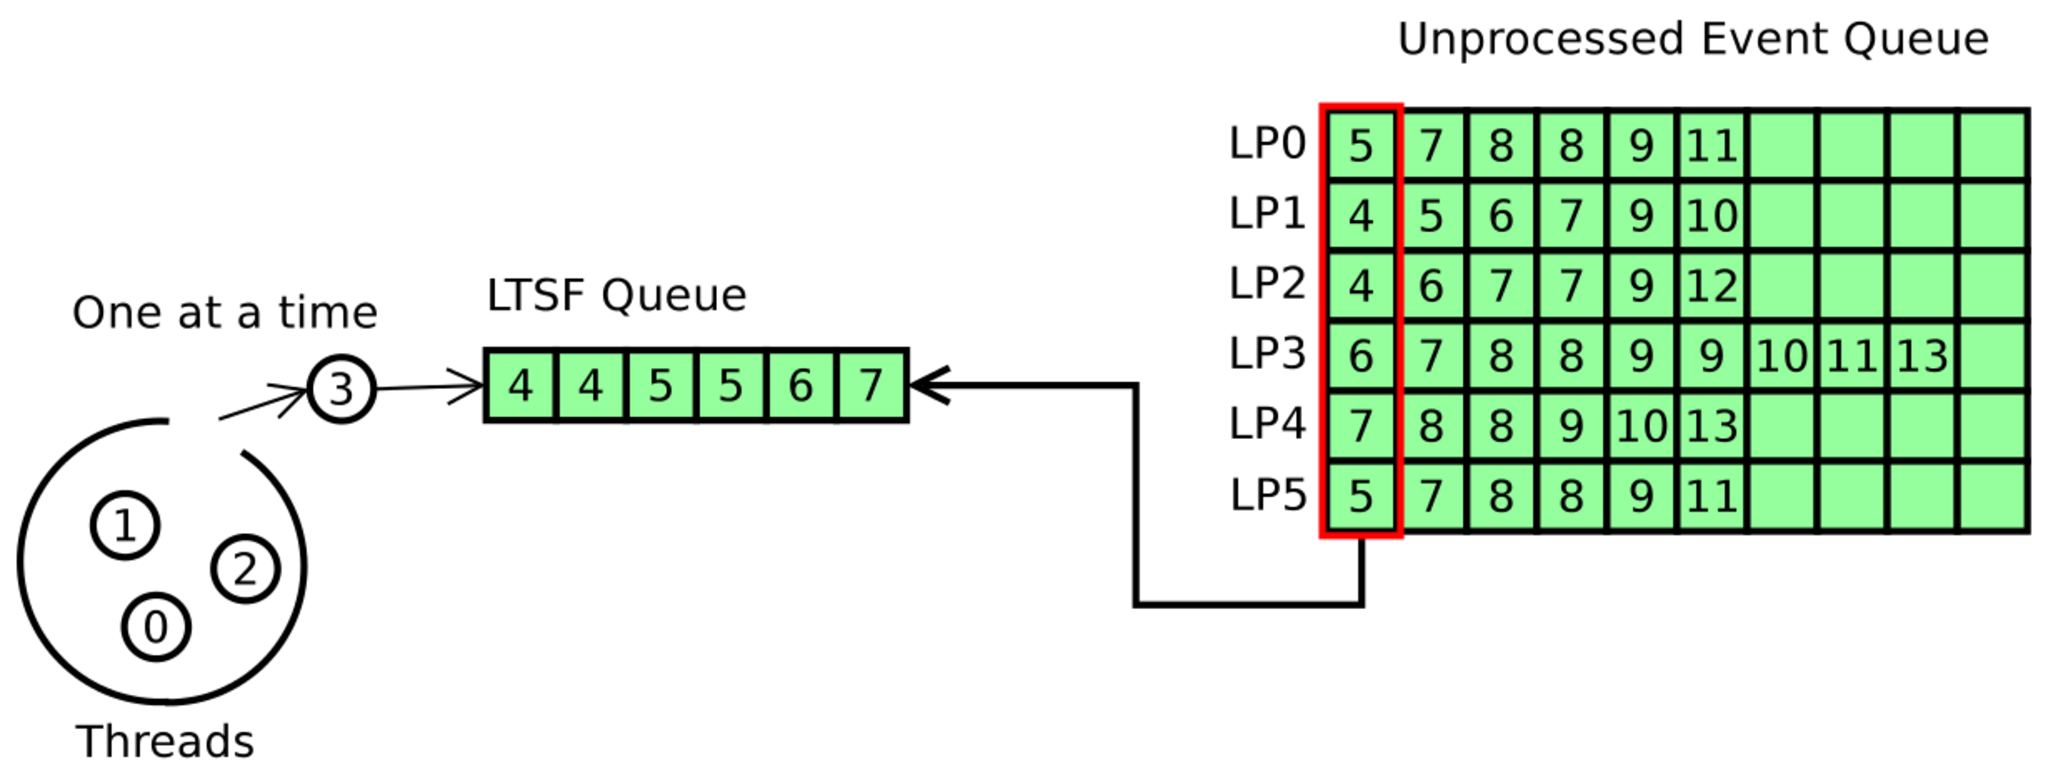
\includegraphics[width=0.65\textwidth,keepaspectratio]{single_ltsf_queue}
    \caption{\textbf{Pending Event Set Scheduling}}\label{fig:singleLTSFqueue}
\end{figure*}

Discrete Event Simulation (DES) models a system's state changes at discrete points in
time.  In a DES model, physical processes are represented by Logical Processes (LPs)
\cite{des_misra}.  For example, in an example epidemic simulation (an example of which is
used in this study), LPs can represent geographical locations containing a subset of the
total population.  The LP's state represents the diffusion of the disease within the
location and the status of the occupants at that location.  Executed Events in this
simulation represent the arrival or departure of individuals to or from that location, the
progression of a disease within an individual at that location, the diffusion of a disease
throughout that location, etc \cite{epidemic}.  To effectively model epidemics, a
significant population size and number of locations needs to be simulated.

%% In general, DES simulators consist of the following data structures \cite{fujimoto}:
%%
%% \begin{itemize}
%%   \item\textbf{Pending Event Set}: contains events that have been scheduled, but not
%%     processed.  Events are retrieved from this structure to be executed.
%%   \item\textbf{Clock}: denotes how far the simulation has progressed.
%%   \item\textbf{State}: describes the state of the system.
%% \end{itemize}
%% 
%% \noindent
%% The state of the simulation can only change upon execution of an event.  During the
%% execution of an event, the simulation: 
%% 
%% \begin{enumerate}
%%   \item retrieves the least time-stamped event from the pending event set,
%%   \item processes the event, 
%%   \item updates the LP's state, and 
%%   \item if necessary, inserts generated events into the pending event set.
%% \end{enumerate}
%% 
%% The need for large simulation models has energized research in Parallel Discrete Event
%% Simulation (PDES).  Events from separate LPs are executed concurrently by one of \emph{N}
%% threads.  Each LPs' events execute in chronological order to ensure local causality
%% constraints are met \cite{fujimoto}.  However, PDES is susceptible to other causality
%% errors.  Optimistically synchronized simulators are the most susceptible to these
%% causality errors.  While conservatively synchronized simulators do not execute events
%% until the system has determined it is safe to do so \cite{fujimoto}, optimistic
%% approaches, such as the Time Warp protocol, detect rather than prevent causal errors. The
%% advantage of optimistic approaches is increased concurrency as events are continually
%% executed until a causal error is detected.
%% 
%% One of the most well-known optimistic protocols is the Time Warp mechanism
%% \cite{fujimoto}.  In addition to the standard DES data structures, each LP in a simulation
%% implementing the Time Warp protocol consists of the following data structures:
%% 
%% \begin{itemize}
%%   \item \textbf{Unprocessed Queue}: contains events that have been scheduled, but have yet
%%     to be executed.  This structure acts as the pending event set for the LP.
%%   \item\textbf{Processed Queue}: records previously executed events.
%%   \item\textbf{Output Queue}: contains event messages sent to other LPs.
%% \end{itemize}
%% 
%% In Time Warp, a causality error occurs if an event message is received containing an event
%% time-stamp smaller than the time-stamp of the previously executed event.  Such an event is
%% known as a \emph{straggler} event.  When a straggler event is received by an LP, that LP
%% must undo all effects of all events executed with a time-stamp greater than that of the
%% straggler event, henceforth referred to as a \emph{rollback}.  During a rollback,
%% prematurely executed events are removed from the processed queue and reinserted into the
%% unprocessed queue after the straggler event.  For every event message in the output queue
%% with an event time-stamp greater than that of the straggler event, an \emph{anti-message}
%% is generated.  Anti-messages are sent to the associated LP of that event and remove the
%% prematurely generated event from the remote LP's queue.
%% Figure~\ref{fig:rollback_stragglerrecvd} shows the scheduling state of the LP as a
%% straggler event is received.  Figure~\ref{fig:rollback_processed} shows the scheduling
%% state of the LP after the rollback is processed \cite{dickman}.
%% 
%% \begin{figure}
%%     \centering
%%     \graphicspath{ {./figures/} }
%%     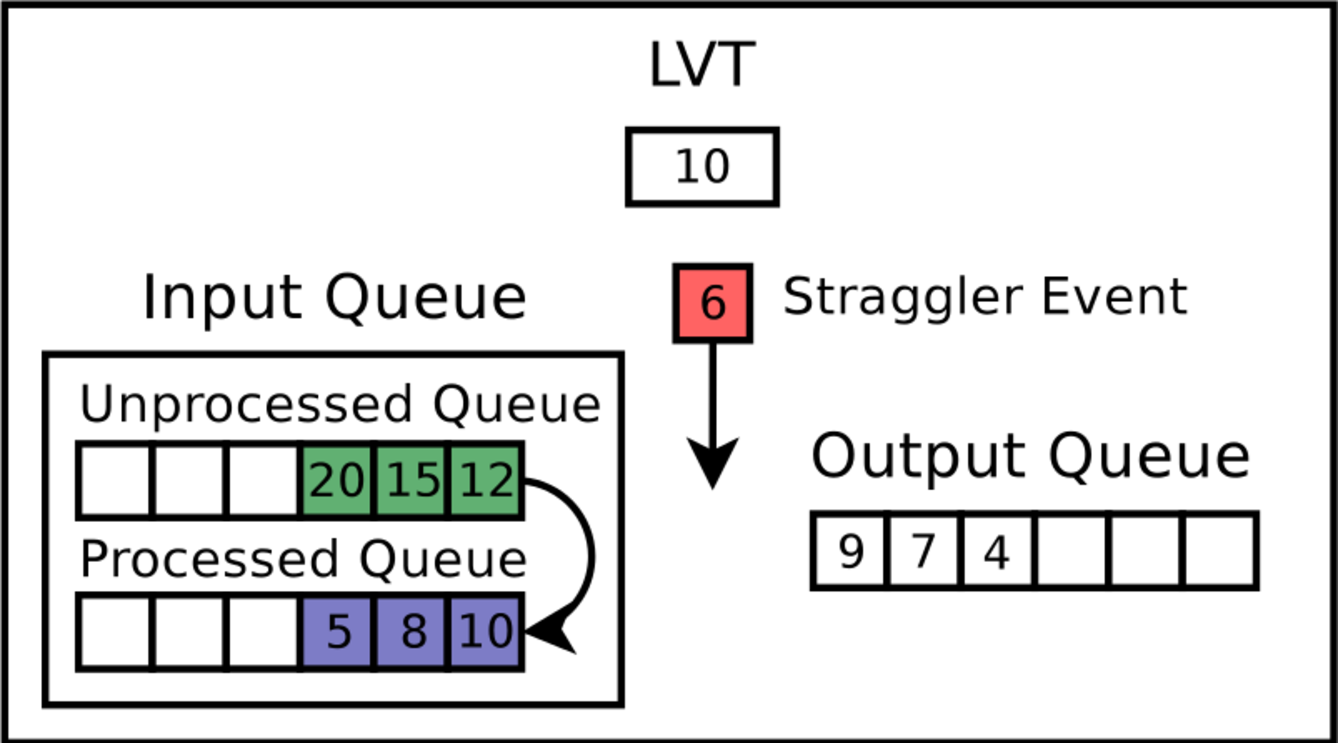
\includegraphics[width=0.5\textwidth,keepaspectratio]{rollback_recv}
%%     \caption{\textbf{LP at the time of a straggler event is
%%         received}}\label{fig:rollback_stragglerrecvd}
%% \end{figure}
%% 
%% \begin{figure}
%%     \centering
%%     \graphicspath{ {./figures/} }
%%     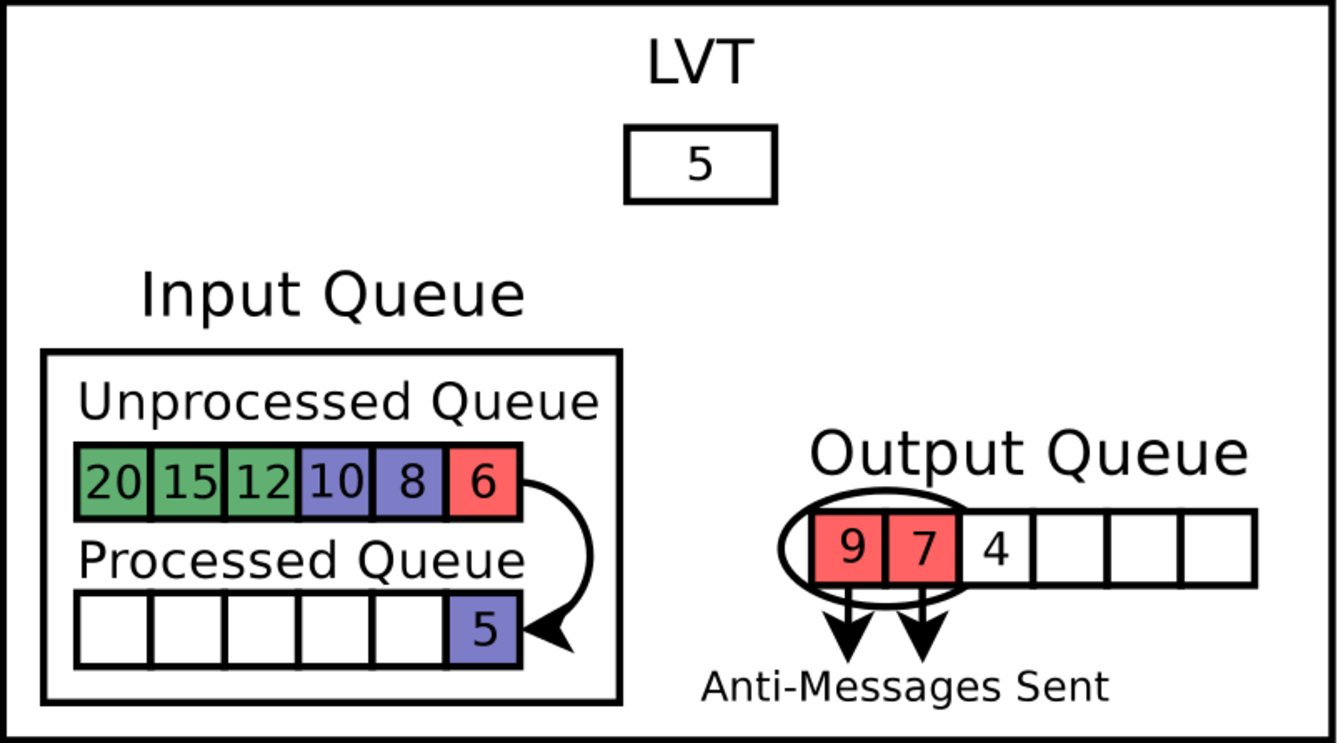
\includegraphics[width=0.5\textwidth,keepaspectratio]{rollback_processed}
%%     \caption{\textbf{LP after a rollback is processed}}\label{fig:rollback_processed}
%% \end{figure}
%% 
%% While rollbacks are a problem in themselves, rollbacks represent another issue relevant to
%% this study; the need to access the pending event set.  When a rollback modifies an LP's
%% local pending event set, the global pending event set must be updated as well.  Any access
%% to the global pending event set is a possible point of contention as only one thread can
%% access this structure at a time.  The implementation and management of the pending event
%% set is crucial to the overall performance of PDES \cite{twpes}.
%% 
%% \subsection{The \textsc{warped} Pending Event Set}

\textsc{warped} is a publicly available Discrete Event Simulation (DES) kernel
implementing the Time Warp protocol \cite{martin,fujimoto}.  It was recently redesigned
for parallel execution on multi-core processing nodes \cite{muthalagu}.  It has many
configuration options and utilizes many different algorithms of the Time Warp protocol
\cite{fujimoto}.

The pending event set is maintained as a two-level structure in \textsc{warped}
(Figure\ref{fig:singleLTSFqueue}) \cite{dickman}.  Each LP maintains its own event set as
a time-stamp ordered queue.  As previously mentioned, each LP maintains an unprocessed
queue for scheduled events yet to be executed and a processed queue to store previously
executed events.  A common Least Time-Stamped First queue is populated with the least time
stamped event from each LP's unprocessed queue.  As the name suggests, the LTSF queue is
automatically sorted in increasing time-stamp order so that worker threads can simply
retrieve an event from the head of the queue.  This guarantees the worker thread retrieves
the least time-stamped event without having to search through the queue. The LTSF queue is
also referred to as the schedule queue in \textsc{warped}; these terms will be used
interchangeably.  

\subsection{Pending Event Set Data Structures}

The implementation of the pending event set is a key factor in the performance of the
simulation \cite{twpes}.  The \textsc{warped} simulation kernel has two functional
implementations: (1) the C++ Standard Template Library (STL) multi-set data structure, and
(2) the splay tree data structure.  The way that these data structures are accessed and,
more importantly, self-adjust will be relevant to how effectively TSX can be used to
access these structures.  Due to space considerations, only performance results with the
multi-set data structure are shown.  Results with splay trees are consistent with those
described in this manuscript.  Interested readers can find those details in \cite{hay-14}.

The sorted STL multi-set data structure is an abstract data structure implemented as a
self-balancing, red-black binary search tree \cite{redblack}.  Look-up, insertion, and
deletion operations performed in a red-black tree with \emph{n} elements are performed in
average O(log n) time.  When insertion or deletion operations are performed, the tree is
rebalanced by a tree rearrangement algorithm and a ``painting'' algorithm taking average
O(1) and O(log n) time respectively.

In the STL multi-set, the lowest value element will always be the left most child node of
the tree.  To access the least time-stamped event at the head of the LTSF queue, multi-set
red-black tree must be traversed to the left most child node.  Any insertion or removal of
events requires that the red-black tree rebalance itself.

\subsection{Worker Thread Event Execution}

Within a \textsc{warped} simulation, a manager thread on each processing node initiates
\emph{n} worker threads at the beginning of the simulation.  It can also suspend inactive
worker threads if they run out of useful work (events in the pending event set).  When a
worker thread is created, or resumes execution after being suspended by the manager
thread, it attempts to lock the LTSF queue and dequeue the least time-stamped event.  If
the worker thread successfully retrieved an event, it executes that event as specified by
the simulation model.  It then attempts to lock the unprocessed queue for the LP
associated with the executed event, and dequeue the next least time-stamped event.  The
dequeued event is inserted into the LTSF queue, which resorts itself based on the event
time-stamps.  An abstract event processing algorithm is shown in
Figure~\ref{workerThreadAlgorithm} \cite{dickman}.  Note that the worker threads perform
many other functions as well.

\begin{figure}
\begin{verbatim}
worker_thread()

  lock LTSF queue
  dequeue smallest event from LTSF
  unlock LTSF queue

  while !done loop

    process event (assume from LPi)

    lock LPi queue 
    dequeue smallest event from LPi
    unlock LPi queue

    lock LTSF queue

    insert event from LPi
    dequeue smallest event from LTSF

    unlock LTSF queue
  end loop
\end{verbatim}
\caption{\textbf{Generalized event execution loop for the worker threads.  Many details
    have been omitted for clarity.}}\label{workerThreadAlgorithm}
\end{figure}

\subsection{Contention}

Only one worker thread can access the LTSF queue at a time.  This creates a clear point of
contention during event scheduling as each thread must first retrieve an event from the
LTSF queue.  The LTSF queue must also be updated when events are inserted into any of the
LP pending event sets.  This occurs when new events are generated or the simulation
encounters a causality error and must rollback.

\begin{figure}
    \centering
    \graphicspath{ {./figures/} }
    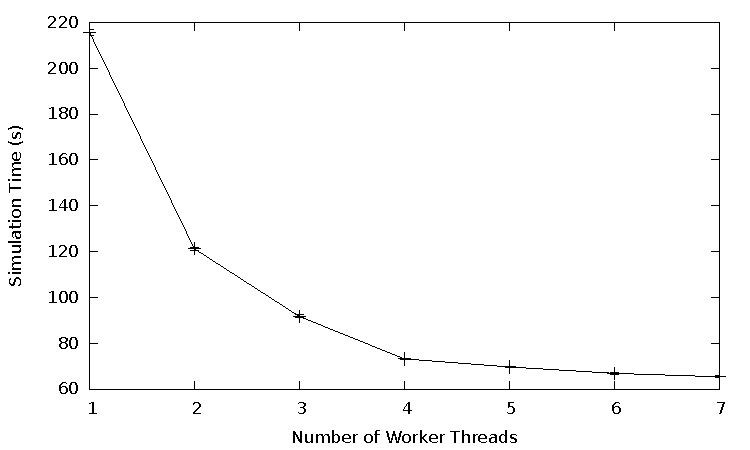
\includegraphics[width=0.5\textwidth,keepaspectratio]{notsx_profile}
    \caption{\textbf{\textsc{warped} Simulation Time versus Worker Thread Count for
        Epidemic Model}}\label{fig:notsx_profile}
\end{figure}

Contention increases with the number of worker threads used to perform the simulation.
The initial \textsc{warped} implementation execution time was measured and analyzed using 1
to 7 worker threads on an Intel i7-4770 with 2-way hyperthreading on 4 processing cores.
These results can be seen in Figure~\ref{fig:notsx_profile}.  It is evident that
performance begins to flatten once the number of worker threads used surpasses four.  This
is attributed to the increased contention for the LTSF queue; with more threads, each
thread has to wait longer for access to the LTSF queue.  The multi-core processor trend
will continue to increase the number of simultaneous execution threads available,
consequently increasing the contention problem.

\subsection{Previous Solutions to Contention}

Dickman \emph{et al} explored the use of various data structures in the
\textsc{warped} pending event set implementation, specifically, the STL multi-set, splay
tree, and ladder queue data structures \cite{dickman}.  A secondary focus of this study
will expand upon the use of splay tree versus STL multi-set data structures; at the time
of this work, the ladder queue implementation was being heavily modified and could not be
included in this study.

Another focus of the Dickman \emph{et al} study was the utilization of multiple LTSF
queues \cite{dickman}.  Multiple LTSF queues are created at the beginning of the
simulation.  Each LP is assigned to a specific LTSF queue as shown in
Figure~\ref{fig:multipleLTSF}.  In a simulation configured with four LPs, two worker
threads, and two LTSF queues, two LPs and one thread are assigned to each queue.  This
significantly reduced contention as each thread could access separate LTSF queues
concurrently.  The initial implementation statically assigned LPs to LTSF queues.  This
resulted in an unbalanced load distribution, leading to an increased number of rollbacks
and reduced simulation performance.  This was corrected using a load balancing algorithm
to dynamically reassign LPs to LTSF queues \cite{dickman}.  This study expands upon the
previous multiple LTSF queue study to evaluate if contention can be reduced even further 
with TSX.

\begin{figure}
    \centering
    \graphicspath{ {./figures/} }
    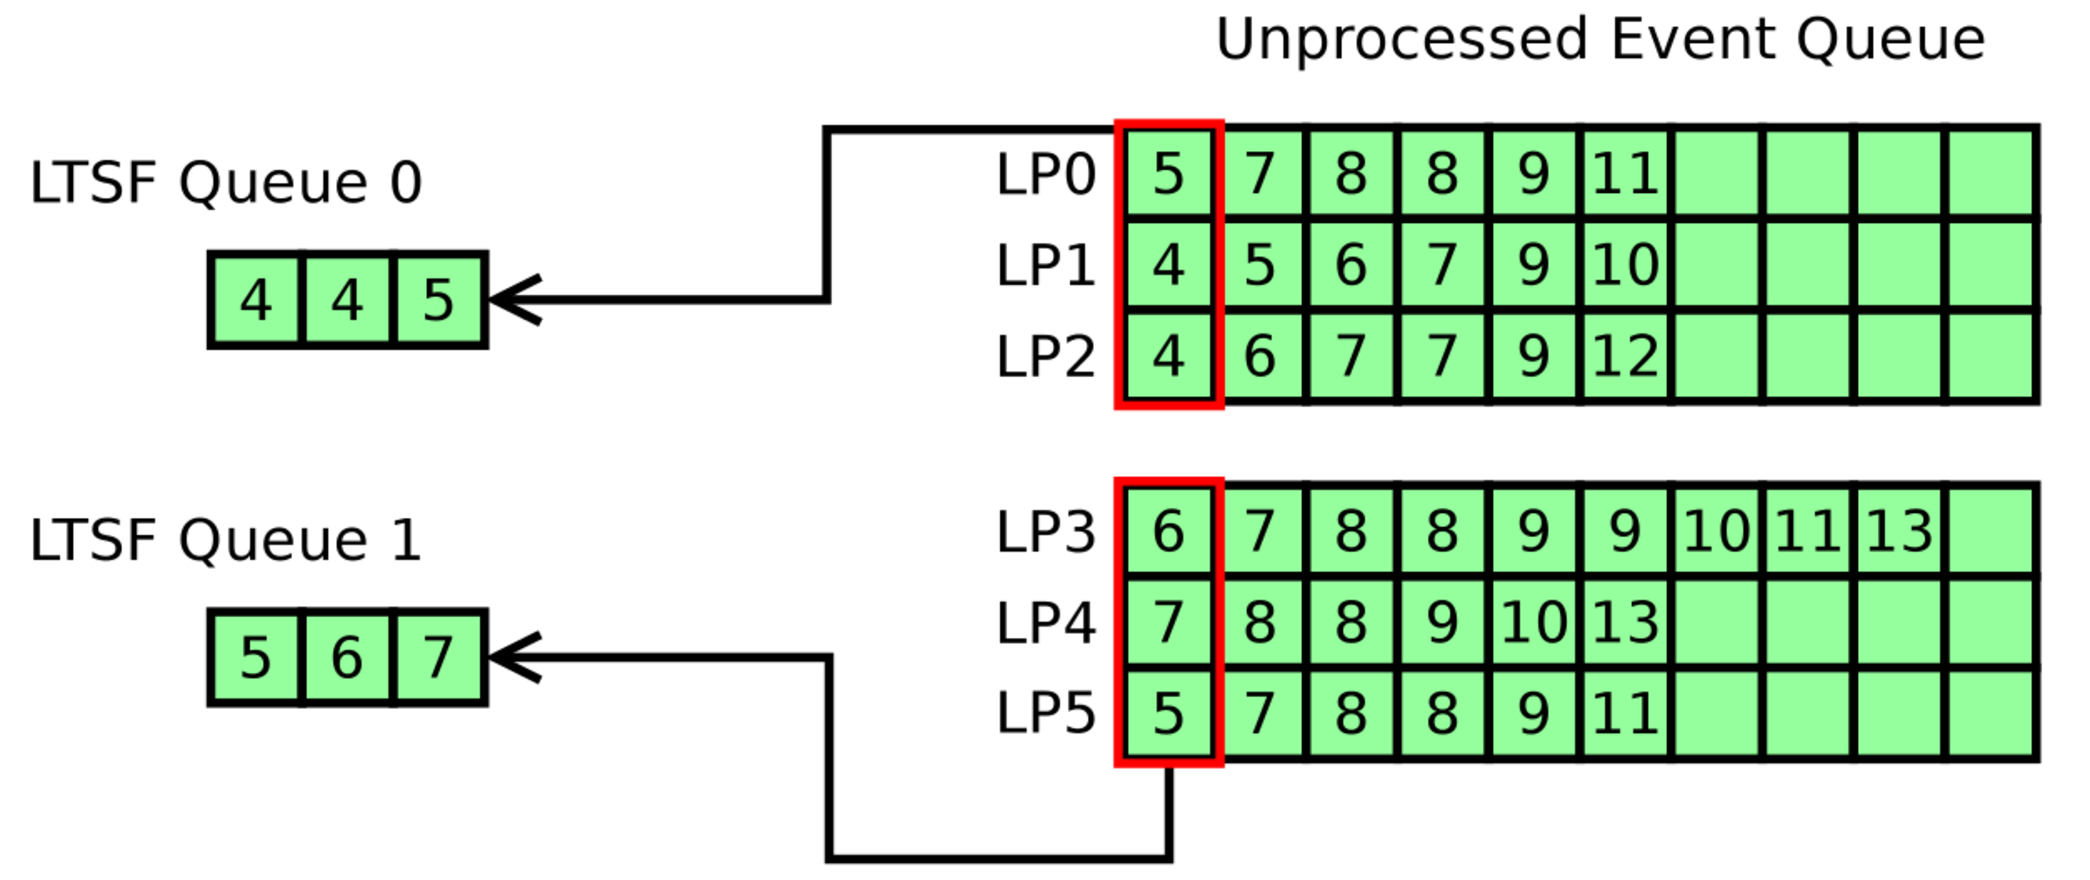
\includegraphics[width=0.5\textwidth,keepaspectratio]{multiple_ltsf}
    \caption{\textbf{Pending Event Set Scheduling with Multiple LTSF
        Queues}}\label{fig:multipleLTSF}
\end{figure}

\subsection{Thread Migration}

Another potential solution to contention is to distribute worker threads that migrate
events from the LPs to subsequent LTSF queues.  That is, in the original scheduling
scheme, worker threads are assigned to a specific LTSF queue.  The worker thread would
insert the next event into the same LTSF it had just scheduled from as seen in
Figure~\ref{workerThreadAlgorithm}.  In this implementation, the worker thread inserts the
next event into a different LTSF queue, based on a circularly incremented counter.  This
approach dynamically reassigns worker threads LTSF queues by migrating the threads to new
LTSF queues.  It also implicitly balances the load between the all the LTSF queues.  The
number of LTSF queues is specified in a configuration file, and has no restrictions as in
the static assignment.

\begin{figure}
\begin{verbatim}
worker_thread()

  i = fetch-and-add LTSF queue index
  lock LTSF[i]
  dequeue smallest event from LTSF[i]
  unlock LTSF[i]

  while !done loop

    process event (assume from LPi)

    lock LPi queue
    dequeue smallest event from LPi
    unlock LPi queue

    i = fetch-and-add LTSF queue index

    lock LTSF[i]

    insert event from LPi into LTSF[i]
    dequeue smallest event from LTSF[i]

    unlock LTSF queue
  end loop
\end{verbatim}
\caption{\textbf{Generalized event execution loop for migrating worker threads.  Many
    details have been omitted for clarity.}}\label{migratinWorkerThreadAlgorithm}
\end{figure}

In a separate (unpublished) study, UC researchers discovered that this implementation
resulted in poor performance on Non-uniform Memory Access (NUMA) architectures.  Jingjing
Wang \emph{et al} also noticed similar performance degradation, which they attributed to
poor memory locality due to the movement of LPs to different threads \cite{numa}.  To
offset these performance hits, a migration count was implemented in this scheme.  Instead
of continuous migration, threads are reassigned to their original LTSF queue after
executing a certain number of events.  The threads will continue to schedule events from
their original LTSF queue for the remainder of the simulation.

\section{\textsc{warped} with TSX}\label{tsx}

This section discusses the various critical sections of \textsc{warped} that use the TSX
mechanism for this study.  As previously mentioned, the primary focus of this study is the
shared LTSF queue.  The LP event queues also modified to use the TSX mechanism.  In
this study, experiments with both the RTM and HLE mechanisms are explored.

The following functions require synchronization to access the LTSF queue:

\begin{itemize}
    \item\texttt{insert()}: copy the least time-stamped event from a specific
        LP's unprocessed queue into the LTSF queue.
  \item\texttt{updatedScheduleQueueAfterExecute()}: find the source LP of the
      previously executed event, and copy the least time-stamped event from that
      LP's unprocessed queue into the LTSF queue using the \texttt{insert()}
      function above.
  \item\texttt{nextEventToBeScheduledTime()}: return the time of the event at the
    beginning of the LTSF queue.
  \item\texttt{clearScheduleQueue()}: clear the LTSF queue.
  \item\texttt{setLowestObjectPosition()}: update the lowest object position
      array. 
  \item\texttt{peek()}: dequeues the next event for execution from the head of
      the LTSF queue.
  \item\texttt{peekEvent()}: if a simulation object is not specified, call \texttt{peek()}. 
  \end{itemize}

Most of these critical sections involve write operations, typically through queuing and
dequeuing events.  Queuing and dequeuing requires the multi-set and splay tree data
structures to readjust themselves thus adding more memory locations to the transaction's
read-set and write-set.  \texttt{nextEventToBeScheduleTime()} is the only critical section
that performs strictly read operations.  Furthermore, many of these critical sections
overlap with critical sections from the unprocessed and processed queues, which are
described below.

%%\subsection{\textsc{warped} Critical Sections}

The functions described above perform a variety of memory operations and any thread can
execute any critical section at any time.  Based on static analysis, there's no way of
knowing which threads will access what structure in what way, hence the need for
synchronization.  However with TSX, functions that do not interfere can execute
concurrently.  TSX tracks read and write memory operations separately in the transaction's
read-set and write-set respectively.  Transactions only interfere if a data conflict
occurs, \emph{i.e.,} a thread attempts to write to a memory location in another
transaction's read-set, or a thread attempts to read a memory location in another
transaction's write-set.

For example, one worker thread calls \texttt{nextEventToBeScheduleTime} to get
the time-stamp of the event at the head of the LTSF queue.  There is a
possibility that a different worker thread is currently updating the LTSF queue
or will attempt to update the LTSF queue while the first worker thread is in
the middle of executing \texttt{nextEventToBeScheduleTime}.  This scenario
necessitates synchronization.  However, in a different scenario, instead of the
second worker thread writing to the LTSF queue, it also calls
\texttt{nextEventToBeScheduleTime}.  Both are read operations and do not
interfere with each other.  TSX recognizes this scenario and allows the worker
threads to execute concurrently, whereas locks force one worker thread to wait
until the other is done with the LTSF queue.

Several similar scenarios can arise during simulation execution.  While there are too many
possible scenarios to identify specifically where TSX can be beneficial, the potential to
expose concurrency through dynamic synchronization is too great to be dismissed.  Note,
there is also no guarantee that TSX will work 100\% of the time; there are several
run-time events that can cause transactions to abort, as well as physical limitations.

\subsection{TSX Implementation}

This section discusses how both TSX interfaces were implemented in \textsc{warped}.

\subsubsection{Hardware Lock Elision (HLE)}

The generic algorithm presented in Figure~\ref{fig:hle_interface} only works for locks
with a binary value, \emph{i.e.,} the lock is free or it is not free.  The \textsc{warped}
locking mechanism assigns the thread number to the lock value to indicate which thread
currently holds the lock.  To comply with this implementation, custom HLE lock acquire and
lock release functions were implemented.  GCC inline assembly functions were developed
appending the appropriate HLE prefixes to the CMPXCHG lock instruction.

These functions are shown in Figures~\ref{hle_inline_xacquire} and
\ref{hle_inline_xrelease}.  The \texttt{\_xacquire()} function loads the value 0xFFFF (the
value indicating the lock is free) into a specific register, then compares the lockOwner
variable with the the previously loaded value to determine if the lock is free.  If the
values are the same, the CMPXCHG instruction will write the value of the threadNumber
variable into the lockOwner variable and return the result.  The \texttt{\_xrelease()}
function loads the value of the lockOwner variable into a specific register, then compares
the threadNumber variable with the previously loaded value.  If the lockOwner value is the
same as the thread number, the cmpxchg writes the value 0xFFFF into the lockOwner variable
to indicate the lock is free.  Of course, if the processor successfully transitions into
transactional execution with the HLE prefixes, the write operations technically never
occur.  They only \emph{appear} to occur to the local thread. Any other thread still sees
the lock as free.

\begin{figure}
\begin{verbatim}
static inline int _xacquire(int *lockOwner, 
    const unsigned int *threadNumber)
{
  unsigned char ret;
  asm volatile("mov $0xFFFF, %%eax\n"
         _XACQUIRE_PREFIX "lock cmpxchg %2, %1\n" 
         "sete %0"
         : "=q"(ret), "=m"(*lockOwner)
         : "r"(*threadNumber) 
         : "memory", "%eax");
  return (int) ret;
}
\end{verbatim}
\caption{\textbf{HLE \texttt{\_xacquire} Inline Assembly Function}}\label{hle_inline_xacquire}
\end{figure}

\begin{figure}
\begin{verbatim}
static inline int _xrelease(int *lockOwner, 
    const unsigned int *threadNumber)
{
  unsigned char ret;
  asm volatile("mov %2, %%eax\n"
         _XRELEASE_PREFIX "lock cmpxchg %3, %1\n"
         "sete %0"
         : "=q"(ret), "=m"(*lockOwner)
         : "r"(*threadNumber), "r"(0xFFFF)
         : "memory", "%eax");
  return (int) ret;
}
\end{verbatim}
\caption{\textbf{HLE \texttt{\_xrelease} Inline Assembly Function}}\label{hle_inline_xrelease}
\end{figure}

\subsubsection{Restricted Transactional Memory (RTM)}

RTM allows the programmer to specify an abort path to be executed upon a transactional
abort.  This allows better tuning of RTM performance.  The RTM algorithm implemented in
\textsc{warped} includes a retry algorithm described below in Figure~\ref{rtm_retry}.
Instead of immediately retrying transactional execution, the algorithm decides when and if
the transaction should be retried based on the condition of the abort.  If the transaction
was explicitly aborted for reasons other than another thread owning the lock, do not retry
transactional execution.  The programmer used the \texttt{\_xabort()} function to
explicitly abort the transaction. If the lock was not free upon entering the transaction,
wait until it is free to retry transactional execution.  If a data conflict occurred, wait
an arbitrary amount of time before retrying.  This offsets the execution of the
conflicting threads in hopes that the conflicting memory operations will be performed at
different times on the next retry.

The RTM retry limit is specified at compile time.  Each data structure
maintains its own retry limit initially set to the global limit.  A back-off
algorithm is used to reduce the retry limit for a specific data structure.  If
the transactions for this data structure abort more often than not, the retry
limit is reduced.  This ideally reduces the number of transaction attempts for
an extended period of time.  If the transaction commit rate increases, the
retry limit increases up to the initial limit specified at compile time.  The
retry limit increases if the commit rate passes the abort to commit rate ratio
threshold.

Furthermore, if transactions for the data structure consistently abort for an extended
period of time with no successful commits, transactional execution is not attempted for
the remainder of the simulation.

\begin{figure}
\begin{verbatim}
while retry count is less than retry limit
  status = _xbegin()

  if status == XBEGIN
    if lock is free
        execute transactional region
    else
        _xabort

  update abort stats

  if transaction will not succeed on retry or 
     _xabort was called due to reasons other 
     than the lock not being free

    break

  else if _xabort was used because the lock 
    was not free

    wait until the lock becomes free to retry

  else if a data conflict occurred
        
    wait an arbitrary amount of time before retrying

  increment retry count
end loop

acquire lock

execute critical section
\end{verbatim}
\caption{\textbf{RTM Retry Algorithm}}\label{rtm_retry}
\end{figure}

\section{Experimental Analysis}\label{eval}

This study compares the performance of the \textsc{warped} simulation kernel using
conventional synchronization mechanisms, Hardware Lock Elision (HLE), and Restricted
Transactional Memory (RTM).  All simulations were performed on a system with an Intel
i7-4770 running at 3.4 GHz with 32GB of RAM.  The average execution time and standard
deviation were calculated from a set of 10 trials for each simulation configuration.  When
comparing synchronization mechanisms, the simulation execution times are compared for the
same LTSF queue and worker thread configurations.  When comparing the LTSF queue
configurations, the multiple LTSF queue configuration execution time is compared with the
execution time of the same configuration with 1 LTSF queue.

The simulation model used to obtain the following results is an epidemic model.  It
consists of 110998 geographically distributed people in 119 separate locations requiring a
total of 119 LPs.  The epidemic is modeled by reaction processes to model progression of
the disease within an individual entity, and diffusion processes to model transmission of
the disease among individual entities.

\subsection{The Default Multi-set Schedule Queue}

The default implementation of the LTSF queue is the STL multi-set data structure.  It is a
self-adjusting binary search tree which keeps the least time-stamped event in the left
most leaf node of the tree.

\subsubsection{Static Thread Assignment}

In the original \textsc{warped} thread scheduling scheme, threads are statically assigned
to an LTSF queue.  Contention will clearly be a problem if the simulation only schedules
from one LTSF queue as every worker thread is assigned to that queue.

The first part of this study compares the performance of the \textsc{warped} pending event
set static thread scheduling implementation using one LTSF queue synchronized with: 

\begin{enumerate}
  \setlength{\itemsep}{-0.05in}
  \item atomic locks, 
  \item HLE, 
  \item RTM with 1 retry, 
  \item RTM with 9 retries, and 
  \item RTM with 19 retries.  
\end{enumerate}

\noindent
These results are shown in Figure~\ref{fig:noThrMig_timeVSthreads_1schq}.  It is clear
that using HLE improves simulation performance, but still suffers from the same rise in
contention as the number of worker threads is increased.  The performance using RTM for
any retry count used is worse than the standard locking mechanism initially.  As the
number of worker threads is increased, the performance using RTM is slightly better than
the standard locking mechanism, but only by about 2 or 3\%.

\begin{figure}
    \centering
    \graphicspath{ {./figures/} }
    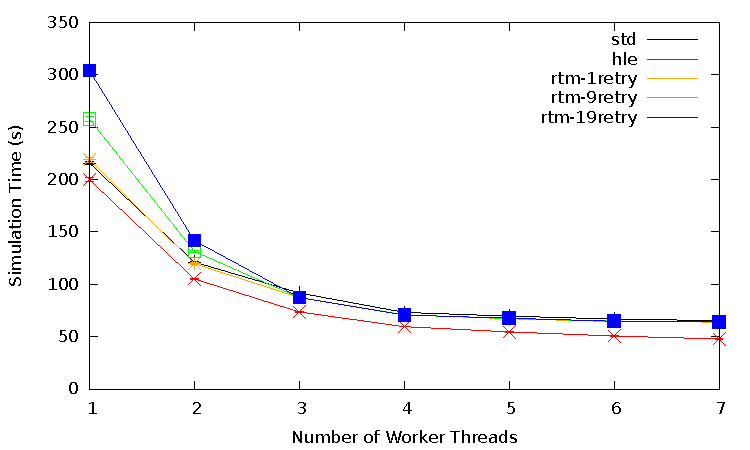
\includegraphics[width=0.4\textwidth,keepaspectratio]{hugeepidemicsim-NOmig-timeVSthreads-multiset-1schQ}
    \caption{\textbf{Performance of a Single Multi-set LTSF Queue}}
    \label{fig:noThrMig_timeVSthreads_1schq}
\end{figure}

It is evident from Figure~\ref{fig:noThrMig_timeVSthreads_1schq} that contention is
increasing as the number of worker threads increases, regardless of the synchronization
mechanism used.  This is somewhat expected as contention is still high for the single LTSF
queue.  Transactional memory exposes concurrency where it can, but some critical sections
simply cannot be executed concurrently.  It should be noted that the performance of HLE
does not flatten quite as much as the other synchronization mechanisms.

The initial solution to alleviate contention for the LTSF queue is the utilization of
multiple LTSF queues.  The data for different numbers of schedule queues is limited by the
necessity to have a number of LTSF queues evenly divisible by the number of worker
threads.  This is because of the way threads are assigned to LTSF queues; if the numbers
are not evenly divisible, the simulation becomes unbalanced.  LPs assigned to a certain
LTSF queue can get far ahead or behind of other LPs on different LTSF queues resulting in
significant rollbacks and thus performance degradation.

Figure~\ref{fig:noThrMig_timeVSthreads_2schedQ} shows the simulation results for varying
worker thread configurations using 2 LTSF queues.  The load balancing restrictions
discussed above restrict the available data for these results.  Each synchronization
configuration yields roughly the same increasing performance trend.  RTM performance seems
to be worse with more retries with a lower worker thread count, but eventually converges
with the single retry scheme.  On the other hand, HLE synchronized simulations
consistently outperform simulations using the standard synchronization.

\begin{figure}
    \centering
    \graphicspath{ {./figures/} }
    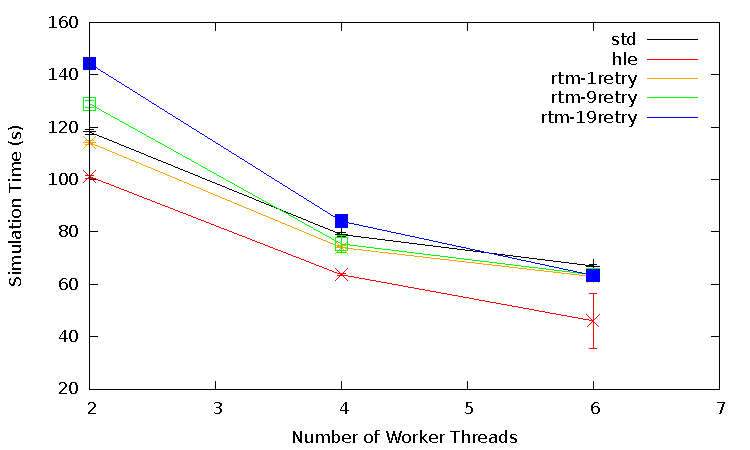
\includegraphics[width=0.4\textwidth,keepaspectratio]{hugeepidemicsim-NOmig-timeVSthreads-multiset-2schQ}
    \caption{\textbf{Performance of Multiple Worker Threads, 2 LTSF Queues}}
    \label{fig:noThrMig_timeVSthreads_2schedQ}
\end{figure}

The LTSF queue count configuration per worker thread configuration results are shown
Figure~\ref{fig:noThrMig_timeVSschq_4threads}.  Using 2 LTSF queues with 2 statically
assigned worker threads appears to alleviate contention.  Using HLE, simulation execution
time was reduced by 13-14\% regardless of the number of LTSF queues used.  RTM improved
performance using only 1 retry, but only by about 1-3\%.  Using any more retries resulted
in worse performance.  Using the standard locking mechanisms, simulation execution time
reduced by about 2.5\% increasing the LTSF queue count from 1 to 2.  With TSX, simulation
execution time reduced by about 4\% when increasing the LTSF queue count from 1 to 2.
While only a small difference, TSX managed to reduce contention a bit more in conjunction
with multiple LTSF queues.

\begin{figure}
    \centering
    \graphicspath{ {./figures/} }
    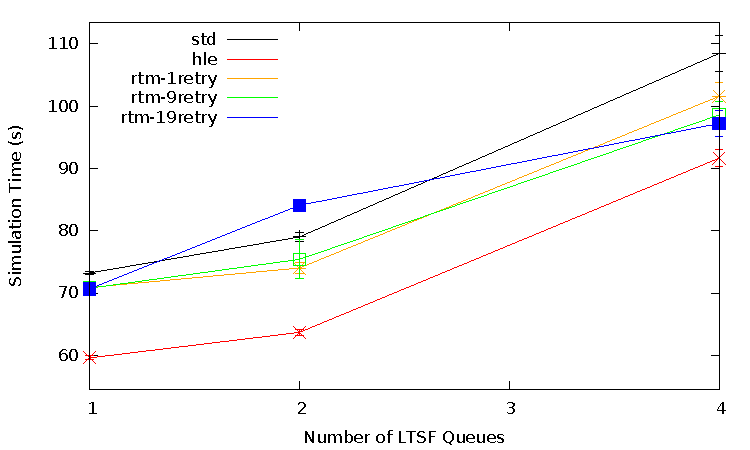
\includegraphics[width=0.4\textwidth,keepaspectratio]{hugeepidemicsim-NOmig-timeVSschedQs-multiset-4thread}
    \caption{\textbf{Performance of Multiple Multi-set LTSF Queues, 4 Statically Assigned Worker Threads}}
    \label{fig:noThrMig_timeVSschq_4threads}
\end{figure}

While TSX substantially improved simulation performance, as much 22\%, simulation
execution time increased as the number of LTSF queues used was increased in other
configurations.  It was noted that these simulations resulted in significantly higher
rollbacks, the most likely cause of the increased execution time.  These poor performance
results could be attributed to the lack of a proper load balancing procedure, which is
addressed with dynamic thread assignment.

\subsubsection{Dynamic Thread Assignment}

Another solution to contention is to distribute worker threads that try to simultaneously
access the same LTSF queue to different LTSF queues.  Worker threads are dynamically
assigned to LTSF queues rather than statically.

The first solution continuously migrates the worker threads to the next LTSF.  That is,
the worker thread processes an event from $LTSF_i$ and then $LTSF_{(i+1)mod n}$ where n is
the number of LTSF queues.  As the worker thread moves among the LTSF queues, the worker
thread also moves the next event from the just processed LP to the next LTSF queue.  This
also helps distribute the critical path of events in the LPs around the LTSF queues.  This
solution implicitly balances the work load between LTSF queues.  Therefore, any number of
LTSF queues can be used with any number of worker threads.

\begin{figure}
    \centering
    \graphicspath{ {./figures/} }
    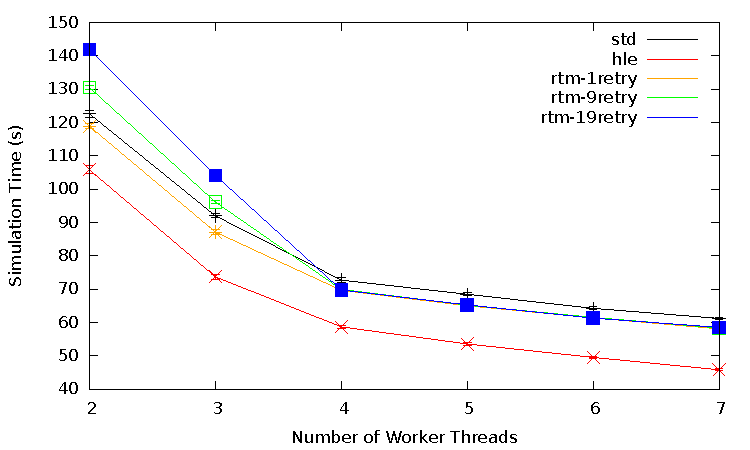
\includegraphics[width=0.4\textwidth,keepaspectratio]{hugeepidemicsim-CONTmig-timeVSthreads-multiset-2schQ}
    \caption{\textbf{Performance of Multiple Dynamically Assigned Worker Threads, 2 LTSF Queues}}
    \label{fig:contThrMig_timeVSthreads_2schQ}
\end{figure}

Figure~\ref{fig:contThrMig_timeVSthreads_2schQ} shows the simulation results for 2 LTSF
queues using the continuous migration scheme as the number of worker threads is varied.
Similarly to the static scheduling scheme, the simulations for each synchronization
mechanism seem to follow almost the same trends.  The more retries the RTM algorithm
attempted, the worse performance was for 2 and 3 worker threads.  However, the number of
retries did not affect the RTM performance for 4 or more worker threads.

\begin{figure}
    \centering
    \graphicspath{ {./figures/} }
    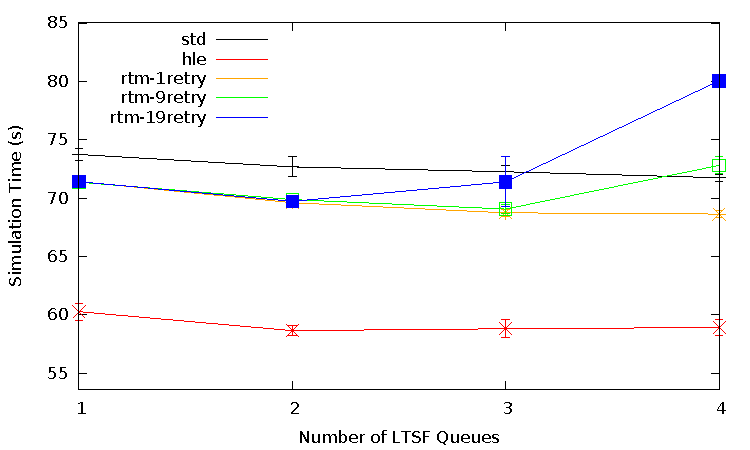
\includegraphics[width=0.4\textwidth,keepaspectratio]{hugeepidemicsim-CONTmig-timeVSschedQs-multiset-4thread}
    \caption{\textbf{Performance of Multiple Multi-set LTSF Queues, 4 Dynamically Assigned Worker Threads}}
    \label{fig:contThrMig_timeVSschq_4threads}
\end{figure}

Simulation execution time decreased slightly by increasing the number of LTSF queue with 4
worker threads (Figure~\ref{fig:contThrMig_timeVSschq_4threads}).  Each multiple LTSF
configuration reduced simulation execution time by 2-3\% when compared to the single LTSF
queue configuration.  The only exception to this trend is the 4 LTSF queue configuration
with HLE; it reduced simulation execution time slightly less than standard locking
mechanisms, but the difference seems trivial.  While RTM performed well for lower LTSF
queue counts, the increased retry counts resulted in worse performance for greater LTSF
queue counts.  In any configuration, HLE still reduces execution time by about 18\%, while
RTM generally generally reduces execution time by about 3-4\% when comparing the two to
standard locking mechanisms.

\begin{figure}
    \centering
    \graphicspath{ {./figures/} }
    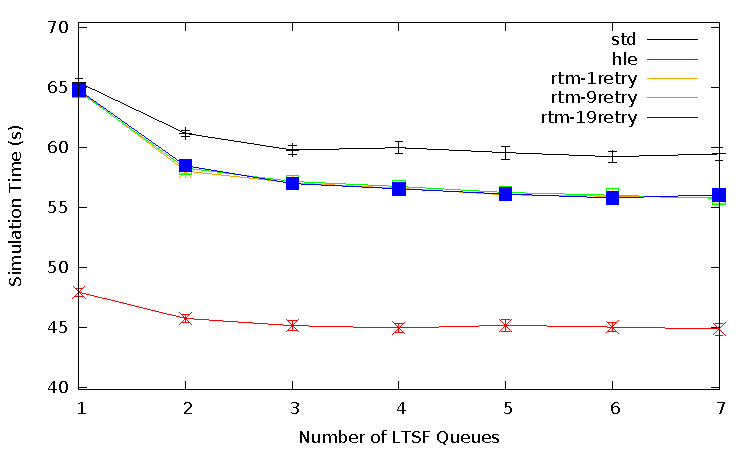
\includegraphics[width=0.4\textwidth,keepaspectratio]{hugeepidemicsim-CONTmig-timeVSschedQs-multiset-7thread}
    \caption{\textbf{Performance of Multiple Multi-set LTSF Queues, 7 Dynamically Assigned Worker Threads}}
    \label{fig:contThrMig_timeVSschq_7threads}
\end{figure}

The final simulation configuration uses 7 worker threads with 1 to 7 LTSF queues
(Figure~\ref{fig:contThrMig_timeVSschq_7threads}).  Using standard locking mechanisms with
multiple LTSF queues reduces execution time from 6\% to 9\% as the number of LTSF queues
is increased.  Surprisingly, HLE only reduces execution time from 3\% to 5\%.  But again,
HLE still well outperforms the standard locking mechanisms by as much as 27\%.  RTM only
outperforms standard locking mechanisms by about 5\%.  However, it becomes much more
effective with more LTSF queues.  Execution time improvements increased from 9\% to almost
14\% when using RTM with increasing LTSF queues counts.

%While the number of LTSF queues is not restricted with this migration
%scheme, it is clear that the performance improvements seen by increasing the
%number of LTSF queues begins to level off after a certain point. Eventually,
%performance stagnates as seen in Figure~\ref{fig:contThrMig_100schedQs}.
%
%\begin{figure}
%    \centering
%    \graphicspath{ {./figures/} }
%%    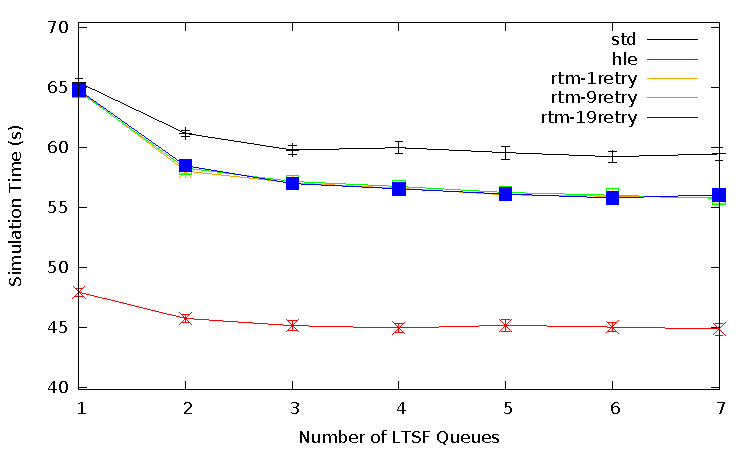
\includegraphics[width=0.4\textwidth,keepaspectratio]{hugeepidemicsim-CONTmig-timeVSschedQs-multiset-7thread}
%    \caption{\textbf{Performance Improvements for Increasing Number of LTSF Queues}}
%    \label{fig:contThrMig_timeVSschq_7threads}
%\end{figure}
%
%It is evident that this scheduling scheme slightly improves performance increasing the
%number of LTSF queues from 1 to 4.  Increasing the number of LTSF queues beyond 4 does not
%seem to significantly improve performance.  The performance of HLE synchronization, while
%still superior, seems to follow the same trend as standard synchronization mechanisms.

As previously discussed, the continuous thread migration approach does not work well for
NUMA architectures due to memory locality issues.  The thread migration scheme was
modified to migrate threads between LTSF queues for the first 50 events a thread executes.
In the first implementation of this scheme, after a thread executes 50 events, it is no
longer reassigned to a different LTSF queue.  It continues to schedule from the same LTSF
queue as it did for the 50th event for the remainder of the simulation.

While the continuous migration scheme is not problematic for the system under test, the
comparison was made to thoroughly evaluate TSX using this scheme as a viable solution to
contention.  TSX may also one day become available on NUMA architectures.  Further testing
would need to be performed, but at least it will be known if this solution has any
significant impact on contention.

\begin{figure}
    \centering
    \graphicspath{ {./figures/} }
    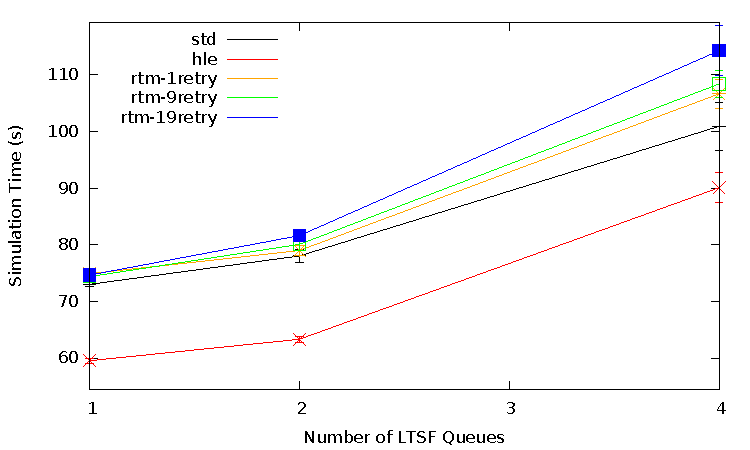
\includegraphics[width=0.4\textwidth,keepaspectratio]{hugeepidemicsim-XEVENTmig-timeVSschedQs-multiset-4thread}
    \caption{\textbf{Simulation Time versus Number of STL Multi-set LTSF Queues for 4
        Worker Threads}}\label{fig:xThrMig_timeVSschq_4threads}
\end{figure}

These results are shown in Figure~\ref{fig:xThrMig_timeVSschq_4threads}.  It is evident
that any static thread to LTSF queue assignment suffers from the same problems.  Except
for the 2 worker thread, 2 LTSF queue and 3 worker thread, 3 LTSF queue configurations,
performance suffers as the number of LTSF queues is increased.  Load balancing becomes an
issue with this migration scheme because worker threads can become unevenly divided among
the LTSF queues leading.

The second implementation attempts to address the load balancing issue by reassigning
worker threads to their original LTSF queues after successfully executing the specified
number of events.  After a thread is reassigned to its original LTSF queue, it continues
to schedule events from that queue for the remainder of the simulation.

Unfortunately, the simulation results were incredibly inconsistent using this scheduling
scheme.  A significant portion of the simulations did not complete execution in the
allotted time.  The longer running simulations experienced significantly higher rollbacks.
When the simulation does appear to run normally, it executes slightly faster than the
strictly static thread assignment scheme.  However, the instability of this migration
scheme made it infeasible to obtain data.

The migration scheme makes a significant difference in contention and load
balancing.  Figures~\ref{fig:migComp_4threads} and
\ref{fig:migComp_7threads} show the comparison of the migration schemes used.
The first implementation of the event limited migration scheme is shown below
since the second implementation performance could not be adequately measured.

\begin{figure}
    \centering
    \graphicspath{ {./figures/} }
    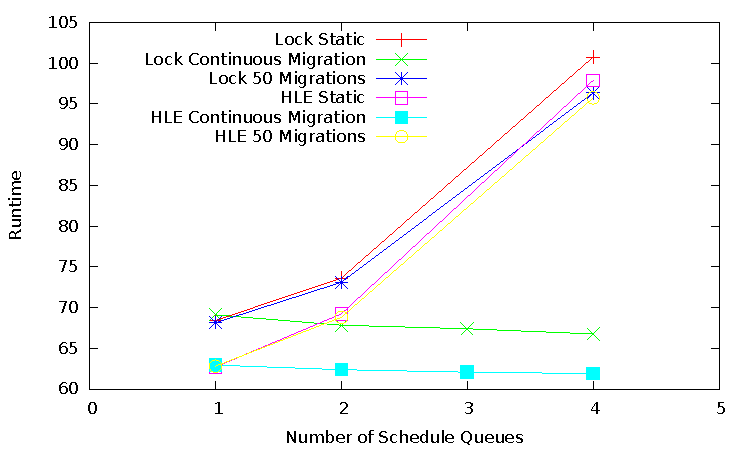
\includegraphics[width=0.4\textwidth,keepaspectratio]{migComp_4threads}
    \caption{\textbf{Comparison of Migration Schemes for 4 Worker Threads with X LTSF
        Queues}}\label{fig:migComp_4threads}
\end{figure}

\begin{figure}
    \centering
    \graphicspath{ {./figures/} }
    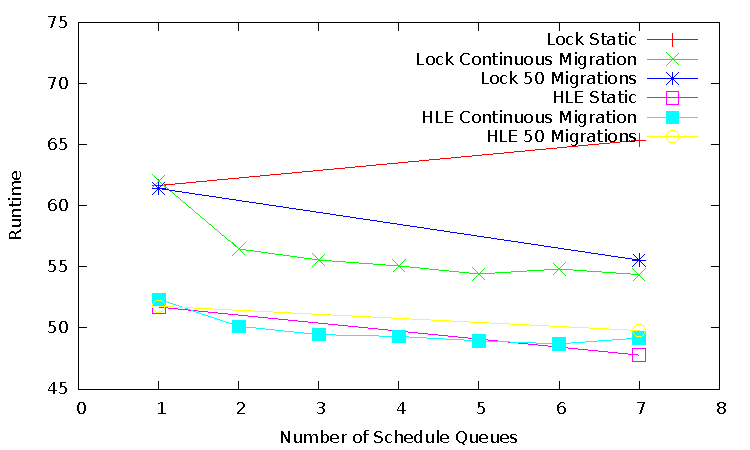
\includegraphics[width=0.4\textwidth,keepaspectratio]{migComp_7threads}
    \caption{\textbf{Comparison of Migration Schemes for 7 Worker Threads with X LTSF
        Queues}}\label{fig:migComp_7threads}
\end{figure}

%% \subsection{The Splay Tree Implementation}
%% 
%% The secondary focus of this study explores how the data structures used to implement the
%% pending event set affects performance.  Because the continuous thread migration scheme
%% already demonstrated significant reductions in contention and implicit load balancing,
%% this thread migration scheme is used to compare the LTSF queue data structure
%% implementations.
%% 
%% The data structure used to implement the LTSF queue will also impact how TSX performs.
%% These results are shown in Figures~\ref{fig:contThrMig_timeVSschq_4threads_msVSst_hle} and
%% \ref{fig:contThrMig_timeVSschq_7threads_msVSst_hle} for simulations using HLE
%% synchronization.  The standard locking based simulations are shown in the same figures for
%% reference.
%% 
%% \begin{figure}
%%     \centering
%%     \graphicspath{ {./figures/} }
%%     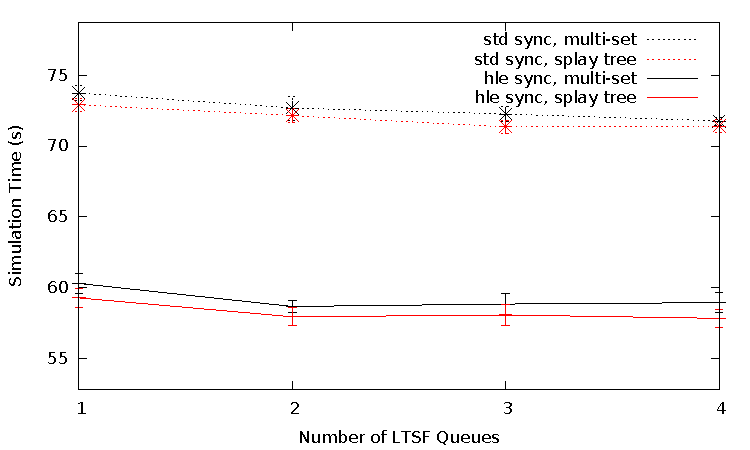
\includegraphics[width=0.4\textwidth,keepaspectratio]{hugeepidemicsim-CONTmig-timeVSschedQs-msVSst-4thread-hle}
%% \caption{\textbf{Multi-Set VS Splay Tree LTSF Queues for HLE
%%      using 4 Worker Threads}}\label{fig:contThrMig_timeVSschq_4threads_msVSst_hle}
%% \end{figure}
%% 
%% \begin{figure}
%%     \centering
%%     \graphicspath{ {./figures/} }
%%     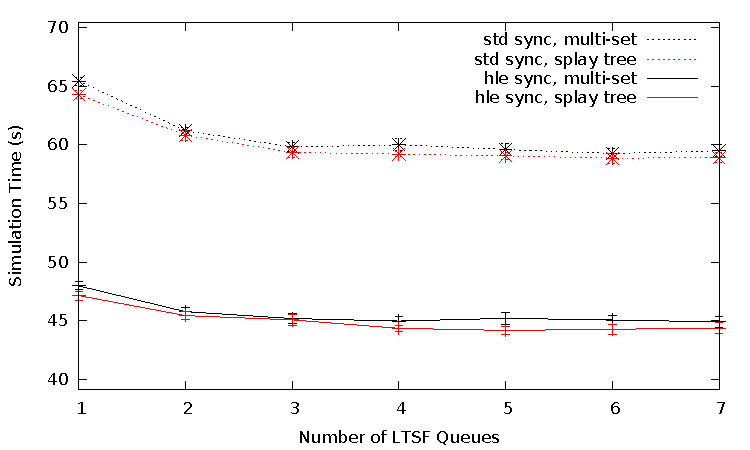
\includegraphics[width=0.4\textwidth,keepaspectratio]{hugeepidemicsim-CONTmig-timeVSschedQs-msVSst-7thread-hle}
%% \caption{\textbf{Multi-Set VS Splay Tree LTSF Queues for HLE
%%      using 7 Worker Threads}}\label{fig:contThrMig_timeVSschq_7threads_msVSst_hle}
%% \end{figure}
%% 
%% It is clear that the simulations using the splay tree LTSF queue consistently execute in
%% slightly less time than the same simulations using the multi-set LTSF queue.  However, it
%% appears that the use of HLE does not alter the performance trends, meaning the
%% implementation of the LTSF queue has little to no effect on the effectiveness of HLE.  It
%% is evident that the performance of the splay tree LTSF queue converges on the performance
%% of the multi-set LTSF queue for configurations using an odd number of LTSF queues with an
%% odd number of worker threads.  In contrast, the splay tree LTSF queue performance seems to
%% slightly diverge from the multi-set LTSF queue performance for configurations using an
%% even number of LTSF queues with an even number of worker threads.
%% 
%% The same comparison is made for the various RTM retry configurations.  These results are
%% shown in Figures~\ref{fig:contThrMig_timeVSschq_4threads_msVSst_rtm1} and
%% \ref{fig:contThrMig_timeVSschq_7threads_msVSst_rtm1}.  The standard locking based
%% simulations are shown in the same figures for reference.
%% 
%% \begin{figure}
%%     \centering
%%     \graphicspath{ {./figures/} }
%%     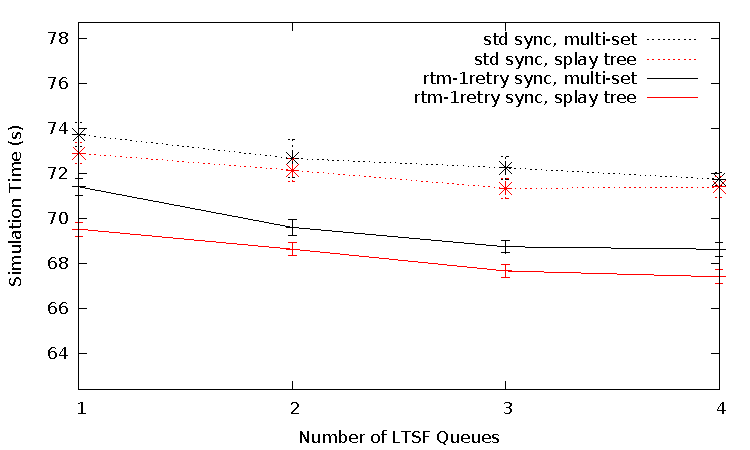
\includegraphics[width=0.4\textwidth,keepaspectratio]{hugeepidemicsim-CONTmig-timeVSschedQs-msVSst-4thread-rtm-1retry}
%% \caption{\textbf{Multi-Set VS Splay Tree LTSF Queues for RTM with 1 Retry
%%      using 4 Worker Threads}}\label{fig:contThrMig_timeVSschq_4threads_msVSst_rtm1}
%% \end{figure}
%% 
%% \begin{figure}
%%     \centering
%%     \graphicspath{ {./figures/} }
%%     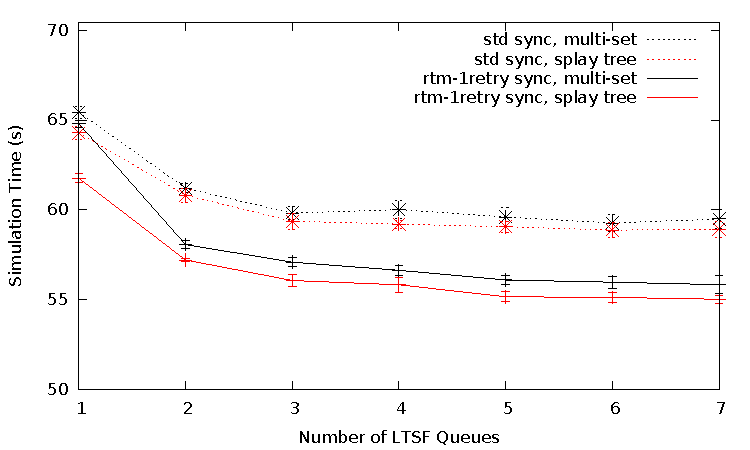
\includegraphics[width=0.4\textwidth,keepaspectratio]{hugeepidemicsim-CONTmig-timeVSschedQs-msVSst-7thread-rtm-1retry}
%% \caption{\textbf{Multi-Set VS Splay Tree LTSF Queues for RTM with 1 Retry
%%      using 7 Worker Threads}}\label{fig:contThrMig_timeVSschq_7threads_msVSst_rtm1}
%% \end{figure}
%% 
%% It is evident that using the splay tree implementation with TSX decreased
%% execution time slightly more than using the splay tree implementation with
%% standard locking mechanisms.  While the difference is small, a 1.5\% improvement
%% versus a 0.5\% improvement, this observation implies that the data structure accessed
%% within critical sections is a factor in the overall effectiveness of
%% transactional memory.  The difference between the performance improvements is
%% fairly consistent.

\subsection{Conclusions}\label{conclude}

This paper explored the use of Intel's transactional memory implementation, Transactional
Synchronization Extensions (TSX) in the multi-threaded \textsc{warped} PDES kernel to
alleviate contention for the pending event set.  The \textsc{warped} pending event set
consists of a global Least Time-Stamped First (LTSF) queue and local event set queues for
each LP.  

Based on the results, it clear that TSX improved the performance of \textsc{warped}.  HLE
consistently shows speedup over conventional synchronization mechanisms.  It even slightly
reduces execution time when the simulation only uses one LTSF queue.  In other
configurations, HLE reduces execution time by as much as 27\% and consistently reduces
execution time by 20\%.

While HLE is the superior synchronization mechanism, RTM still showed increases in
performance, generally by about 5\%.  It also works with multiple LTSF queues better than
HLE.  This is most likely attributed to the retry algorithm.  HLE transactions only have
one chance to execute a transaction. If contention is high at certain times, the
transaction will most likely abort.  The RTM retry algorithm uses abort information to
decide when to retry transactional execution, rather than immediately aborting the
transaction or using conventional synchronization mechanisms.  RTM might not perform as
well as HLE due to the overhead associated with RTM.  The retry algorithm requires abort
statistics to be calculated and maintained which adds a bit more overhead to RTM.

TSX is not likely to allow simultaneous access to the same LTSF queue when the structure
is being written.  TSX synchronization mechanisms also appear to be more expensive.
The performance increases seen with TSX are most likely result from the concurrent
execution of critical sections involving only read operations.  Furthermore, some critical
sections bypassed their write operations under certain conditions.  For example, a check
was performed within a critical section to ensure the LTSF queue was not empty.  If the
queue was empty, the critical section ended without performing any operations.  With
standard synchronization, this critical section would still suffer from the locking
overhead, even though it wasn't necessary.  With TSX synchronization, the check could
potentially execute concurrently with another thread.  The same scenarios apply to each
LP's processed and unprocessed queue.  Overall, TSX reduced unnecessary contention.

%% The splay tree data structure performs better than the multi-set regardless of
%% synchronization.  When synchronized with TSX, the splay tree implementation seemed to
%% reduce execution time a bit more.  The way in which data structures are accessed is a
%% factor in how effectively transactional memory operates.  

In conclusion, TSX significantly improves simulation performance for the \textsc{warped}
PDES kernel.  While other solutions to contention showed improvements in performance, they
were not nearly as significant as TSX, especially HLE.  TSX only showed slight
improvements in its own performance when combined with these other solutions.  Regardless,
TSX is powerful solution to contention.

%% \section*{Acknowledgments}
%% 
%% Support for this work was provided in part by the National Science Foundation
%% under grant CNS--0915337.

\bibliographystyle{abbrv}
\bibliography{refs}

\end{document}
